\subsection{Opis hipotezy}\label{opis-hipotezy}

\textbf{Numer:} 9\\\textbf{Nazwa:} Wypadki a wiek
kierowców\\\textbf{Treść:} Najwięcej wypadków będzie powodowanych przez
kierowców młodych ze względu na brawurę i brak doświadczenia.

\subsection{Wyniki związane z
hipotezą}\label{wyniki-zwiazane-z-hipoteza}

\textbf{Wiek kierowcy}

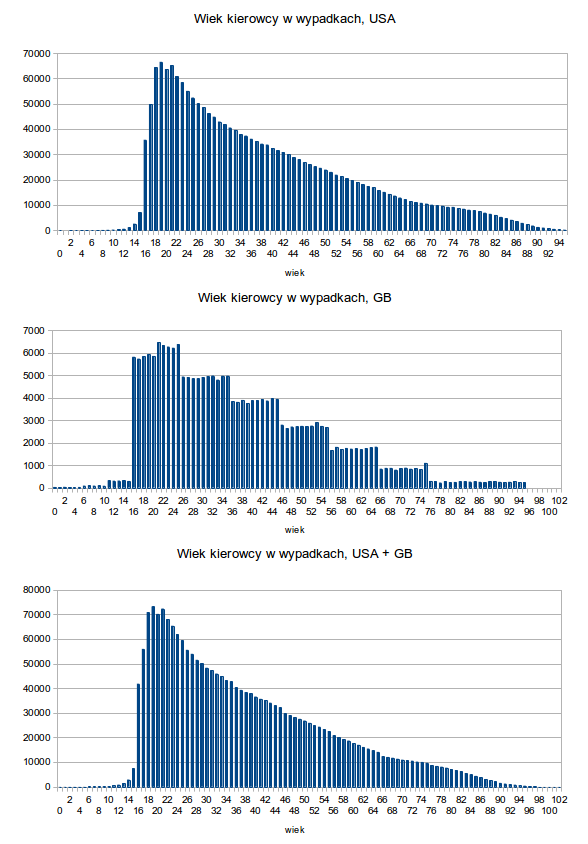
\includegraphics[width=0.9\textwidth]{images/statistics/driver_age.png}

\textbf{Wiek uczestników wypadku}

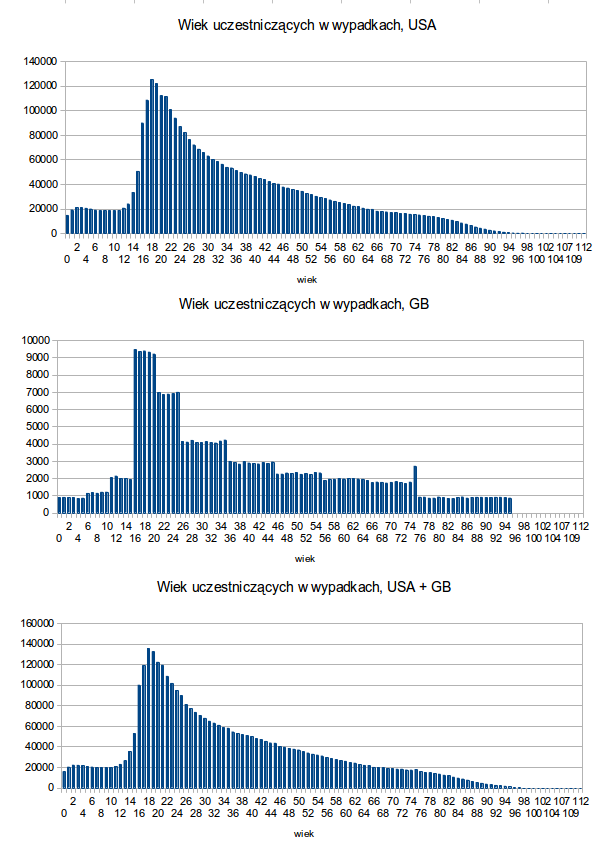
\includegraphics[width=0.9\textwidth]{images/statistics/person_age.png}

\subsection{Weryfikacja i wnioski}\label{weryfikacja-i-wnioski}

Hipoteza potweirdziła się, największa liczba wypadków jest wśród młodych
kierowców. Jest to związane przede wszystkim z brakiem doświadczenia i
umiejętności a także często z brawurą i zbytnią pewnością siebie.

Niestety z powodu braku dokładnych danych o wieku w danych z Wielkiej
Brytanii a jedynie przedziałów wiekowych, nie widać różnicy między
wiekiem, w którym kierowcy mogą rozpocząc kierowanie pojazdami. Widać ze
w USA jest to 16 - 18 lat (zależnie od satnu), jednak dla danych z
Wielkiej Brytanii mozemy stwierdzić jedynie, że jest to gdzieś w
przedziale 16 - 21.

Analiza wieku ofiar pokazuje, poprzez swoje podobieństwo do wykresu dla
kierowców, że często kierowca jest jedyną osobą w pojeździe bądź też
podróżuje ze swoimi rówieśnikami.
